
\section{{\prg mcdisp} - the Calculation Program for Magnetic Excitations}\label{mcdisp}

For a given field $\mbf H$ and temperature $T$ the dynamics of the magnetic system
can be calculated by the program {\prg mcdisp\index{mcdisp}}. It requires as input files
the {\prg mcphas.j\index{mcphas.j}} and single ion input files. In addition, the input file
{\prg mcdisp.par\index{mcdisp.par}} and {\prg mcdisp.mf\index{mcdisp.mf}} are needed (see description below).

\begin{description}
\item [\prg mcdisp [options]][file.mf]]  
      calculates the dispersion of magnetic excitations
	  needs as input file a {\prg file.mf} (default {\prg mcdisp.mf\index{mcdisp.mf}})
				and {\prg mcdisp.par\index{mcdisp.par}}.  Creates  
				files {\prg ./results/mcdisp.qom} and {\prg ./results/mcdisp.qei}
				containing the dispersion of the magnetic excitations and the neutron
				scattering intensity. 
				
				Options are:
				 \begin{itemize}
				\item Option {\prg -max} restricts the single ion susceptibility
				used to maximum of  the n lowest lying transitions, starting
				from the ground state (useful to save calculation time).
--
			        Note that by options {\prg -minE} and {\prg -maxE}
				also an energy interval may be given (minE,maxE):
				Single ion transitions with energies outside this
				energy interval are not considered.
                                               \item option {\prg -d} forces mcdisp to do calculation of intensities in dipole approximation only				
				\item Option {\prg -r} is used to calculate the energy dependence
				of the cross section via the dynamical susceptibility (see below).
				\item To create an output
				of the Fourier transform ${\mathcal J}({\mbf Q})$ use option
				{\prg -jq}. 
				\item {\prg -v} option is to display\index{display} more information.
                                
				\item Option {\prg -a} can be used to avoid overwriting output files in results, new results
				are appended.
								
				\item Option {\prg -c}  can be used to create  a single ion
				transition file {\prg ./results/mcdisp.trs}, which contains
				all single ion transitions used in the calculation. This file can
				be edited (uncommenting single ion transitions which should not
				by used by a \# sign at the beginning of the line)
				and then the program can be restarted using the 
				\item  option {\prg -t} to
				read the single ion transition file {\prg ./results/mcdisp.trs} and
				calculate energies and neutron intensities.
				\end{itemize}
\item [\prg mcdispit [options]][file.mf]]  same as {\prg mcdisp}, but no graphic window
\end{description} 

\subparagraph{example of input file {\prg  mcdisp.mf}}
this file contains temperature $T$, the external field $H$ and
the effective fields on the different sites:

\begin{verbatim}
# Parameter file  mcdisp.mf - read by mcdisp version 3.0
#<!--mcdisp.mcdisp.mf>
#*********************************************************************
# mcdisp - program to calculate the dispersion of magnetic excitations
# reference: M. Rotter et al. J. Appl. Phys. A74 (2002) 5751
#*********************************************************************
#'T'             temperature T
#'Ha' 'Hb' 'Hc'  magnetic field
#'n'             number of atoms in magnetic unit cell
#'nofatoms'      number of atoms in primitive crystal unit cell
#'nofcomponents' dimension of moment vector of a magnetic atoms
T=2 Ha=0 Hb=0 Hc=0 n=10 nofatoms=2 nofcomponents=3
 0.0000 0.0000 0.0000 0.0000 0.0000 0.0000 0.0000 0.0000 0.0000 0.0000
 0.2708 0.3354 -0.3354 -0.2708 0.2947 -0.2708 -0.3354 0.3354 0.2708 -0.2947
 0.0000 0.0000 0.0000 0.0000 0.0000 0.0000 0.0000 0.0000 0.0000 0.0000
 0.0000 0.0000 0.0000 0.0000 0.0000 0.0000 0.0000 0.0000 0.0000 0.0000
 0.2708 0.3354 -0.3354 -0.2708 0.2947 -0.2708 -0.3354 0.3354 0.2708 -0.2947
 0.0000 0.0000 0.0000 0.0000 0.0000 0.0000 0.0000 0.0000 0.0000 0.0000
\end{verbatim}

The file {\prg mcdisp.mf\index{mcdisp.mf}} can be easily set up by using the program {\prg %%@
setup\_mcdisp\_mf\index{setup\_mcdisp\_mf}} or alternatively by the program {\prg spins\index{spins}} 
described in section~\ref{spins}.

\subparagraph{example of input file {\prg mcdisp.par\index{mcdisp.par}}}

{\footnotesize
\begin{verbatim}
# Parameter file  mcdisp.par - read by mcdisp version 3.6
#<!--mcdisp.mcdisp.par>
#*********************************************************************
# mcdisp - program to calculate the dispersion of magnetic excitations
# reference: M. Rotter et al. J. Appl. Phys. A74 (2002) 5751
#*********************************************************************
#
# mcdisp calculates the neutron scattering cross section dsigma/dOmegadE' [barn/sr/meV/f.u.]
#           f.u.=crystallogrpaphic unit cell (r1xr2xr3) for inelastic and diffuse scattering
#
# depending on what is kept constant it follows either kf or ki (1/A)
#!kf=3.474
# 
# emin and emax define the energy range in which neutron intensities are calculated
# for full calculation of the dynamical susceptibility (option "-r", inversion of the MF-RPA equation 
# for each point in Q-omega space) the minimum and maximum energy has to be given (energy stepwidth is 
# equal to the parameter epsilon given in the command line after "-r")
#
#!emin=0.1
#!emax=80
#
# optional parameter is extended_eigenvector_dimension
# which is used to define, how many components of the
# eigenvector should be in the ouput to file mcdisp.qee
# important for charge density movies, e.g.(i) for module so1ion
#  - f electrons - chargedensity fluctuation needs coefficients
#  l=3, i.e. eigenvector should be extended to 3+5+7+9+11+13=48,
#  (ii) for module ic1ion with f-electrons eigenvector has to be
#  extended to 6+5+7+9+11+13=51 (here there are 6 components for 
#  all spin and orbital moments), (iii) for module ic1ion and d-
#  electrons l=2 it suffices 6+5+7+9=27 
#!extended_eigenvector_dimension=3
#
# It follows either 
#
# (i) a Q vector mesh to be mapped in the calculation
#!hmin=1 hmax=24 deltah=1
#!kmin=0 kmax=0 deltak=1000
#!lmin=0 lmax=0 deltal=1000
#
# or 
# (ii) file(s) containing list of Q vectors with (optional) energies of observed excitations to be fitted
# h k l [E1(meV) E2(meV) ...]
#
# hklfile=file1
# hklfile=file2
# ...
#
# or
# (iii) a list of Q vectors with (optional) energies of observed excitations to be fitted
# h k l [E1(meV) E2(meV) ...]
0.297 0.297 0 11 
0.311 0.311 0 10 


\end{verbatim}
}

this file describes, which $q$ vector range to
calculate:

\begin{verbatim}
#   q vector range (qmin qmax deltaq)
hmin=0 hmax=0.2 deltah=0.01
kmin=1 kmax=1 deltak=0.05
lmin=0 lmax=0 deltal=0.02
\end{verbatim}

alternatively these lines can be commented and a
list of reflections can be given in {\prg mcdisp.par\index{mcdisp.par}}, the
program {\prg mcdisp\index{mcdisp}} then calculates only 
the excitation energies at these reflections and (if measured
energies are given) computes a standard deviation
and prints
this deviation to stdout as ''sta=3120.31'' [this can directly
be used by fitting program such as {\prg simannfit\index{simannfit}}].

The standard deviation is calculated by taking for a set of measured energies (at a 
given q-vector) the squared sum of differences to the nearest
calculated energy. Statistical weighting as given by the user in {\prg mcdisp.par}
for each q-vector is applied. If the weighting is less than zero, the 
inverse squared sum of differences to the nearest
calculated energy is taken (''antipeak'', this is useful in order to 
tell the program, that there is no peak at this energy).
In addition to the standard deviation ''sta'' some other quantitites are calculated and 
may be used in fitting experimental data:

\begin{eqnarray}
{\rm sta}                              & =& \sum_i |weight(i)|*[Eexp(i) - nearestEcalc(i)]^{[2*sign(weight(i))]}\\
{\rm sta\_int   }                       & = &\sum_i |weight(i)|*[Eexp(i) - nearestEcalc_{\rm with %%@
Int>0.1mb/srf.u.}]^{[2*sign(weight(i))]}\\
{\rm sta\_without\_antipeaks }           & =& \sum_{i, weight(i)>0}  weight(i)*[Eexp(i) - nearestEcalc(i)]^2\\
{\rm sta\_int\_without\_antipeaks }       & =&\sum_{i,weight(i)>0}  weight(i)*[Eexp(i) - nearestEcalc_{\rm with %%@
Int>0.1mb/srf.u.}]^2\\
{\rm sta\_without\_weights }              &=& \sum_i [Eexp(i) - nearestEcalc(i)]^{[2*sign(weight(i))]}\\
{\rm sta\_int\_without\_weights}          & =&\sum_i [Eexp(i) - nearestEcalc_{\rm with %%@
Int>0.1mb/srf.u.}]^{[2*sign(weight(i))]}\\
{\rm sta\_without\_antipeaks\_weights}    & = &\sum_{i, weight(i)>0}[Eexp(i) - nearestEcalc(i)]^2\\
{\rm sta\_int\_without\_antipeaks\_weights}& =& \sum_{i, weight(i)>0} [Eexp(i) - nearestEcalc_{\rm with %%@
Int>0.1mb/srf.u.}]^2\\
\end{eqnarray}



If option {\prg -r 0.032} is used, the energy dependence of 
the scattering cross section is calculated within limits [emin,emax].
The number, 0.032 in our case, indicates the imaginary part of $\omega$ 
in units of meV (see equations
in section~\ref{formalism}). Setting it zero would lead to numerical
divergencies, choosing it to large leads to large half widths of the calculated 
peaks. 
 Output
is stored in output file {\prg mcdisp.dsigma}.

The output files of program {\prg McDisp} are 

\begin{quote}
\item[{\prg mcdisp.trs}:] contains all single ion transitions with strengths $\gamma$ 
and neutron intensities.
\item [{\prg mcdisp.qom}:] Contains the energies of the modes and scattering cross sections  for each mode 
calculated using the DMD algorithm described in section~\ref{intapprox}
\item[{\prg mcdisp.qei}] energies and neutron scattering intensities calculated by the DMD algorithm, if 
        the energy of a mode is outside interval  [emin,emax] the value -1 is output for the intensity.
\item[{\prg mcdisp.qev}] eigenvectors (relative phase and amplitudes) for the modes
\item [{\prg mcdisp.dsigma}(only created with option {\prg -r}):] Contains the energy dependence of the scattering cross %%@
section
calculated according to section~\ref{formalism} within the energy range specified by [emin,emax] given in {\prg %%@
mcdisp.par}. 
\item [{\prg mcdisp.dsigma.tot}:] sum of intensities in interval  [emin,emax].  For option {\prg -r} : Sum of intensities calculated in {\prg %%@
mcdisp.dsigma}.
\end{quote}

\vspace{1cm}
{\em Exercises:}
\begin{itemize}
\item Type {\prg mcdisp -max 3 -i} to
calculate the dispersion of magnetic excitations for NdCu$_2$.
and inspect the results
{\prg examples/ndcu2b\_new/results}.
Which  transition has the largest intensity ?
\end{itemize}

\subsection{Viewing the results of McDisp}

\begin{quote}
\item [\prg displaybubbles\index{displaybubbles} ] produces a plot of the calculated dispersion on screen, which is 
                       automatically updated when the file changes. In contrast to the normal
		       display\index{display} program the radius of the symbols is increased according to
		       the values of a radius column (in our case intensity column in file
		       mcdisp.qui). Use as {\prg displaybubbles\index{displaybubbles} 
		       xcol ycol rcol filename} - i.e. for displaying the dispersion along
		       {\em h} type {\prg displaybubbles\index{displaybubbles}  5 8 9 mcdisp.qei}. 
\item [\prg displaycontour\index{displaycontour}] displays contour plot of scattering intensity - use as
                       {\prg displaycontour\index{displaycontour} xcol ycol zcol filename} - i.e. for displaying
		       the intensity versus {\em hk} type {\prg displaycontour\index{displaycontour} 5 6 8 mcdisp.dsigma.tot}
		       (see fig.~\ref{diffus})
\item [\prg spectrum]  reads mcdisp.qom or mcdisp.dsigma and produces spectrum
                       as an xy file, use as {\prg spectrum h k l filename}
\end{quote}

\subsection{Formalism}
\label{formalism}

This section is describes the formalism used in the calculation of the magnetic excitations. Because the
procedure is not standard, we list the most important formulas.

The double differential
inelastic neutron cross section of magnetic excitations has been given in~\cite{jensen91-1}~\footnote{\em %%@
http://www.nbi.ku.dk/page40667.htm} (compare also equations (\ref{dsdode}) and (\ref{smag}))

\begin{eqnarray}\label{int}
\frac{d \sigma_{\rm mag}^{\rm inel}}{d\Omega dE'}&=&N \frac{k'}{k} \left(\frac{\hbar \gamma e^2}{m_e c^2}\right)^2
%\sum_{\mbf Q} \delta_{\vec\kappa,\mbf Q}
\sum_{\begin{array}{c} \alpha \beta \\ s s' \\ \end{array}}
(\delta_{\alpha\beta}-\hat Q_{\alpha} \hat Q_{\beta})
\{\frac{1}{2} g_J F(Q)\}_s \{\frac{1}{2} g_J F(Q)\}_{s'}
 \times \nonumber  \\
&&\times e^{-W_s(Q)- W_{s'}(Q)} 
\frac{S_{ss'}^{\alpha\beta}({\mbf Q},\omega)}{2\pi \hbar N_b}  \nonumber \\
S_{ss'}^{\alpha\beta}({\mbf Q},\omega) &=&
\frac{2 \hbar}{1-e^{-\hbar\omega/kT}} \chi_{\alpha\beta}^{,,ss'}({\mbf Q},\omega) \\ \nonumber
\chi_{\alpha\beta}^{,,ss'}({\mbf Q},\omega)&=&
\frac{1}{2i}\left[
\chi_{\alpha\beta}^{ss'}({\mbf Q},\omega)-
\chi_{\beta\alpha}^{*s's}({\mbf Q},\omega)
\right]
\end{eqnarray}

 
In (\ref{int}) 
$N$ denotes the number of magnetic atoms in the sample, $\mbf k$ and $\mbf k'$ the wave vector of the incoming and
scattered neutron, respectively.
The total magnetic cross section is $4\pi\left(\frac{\hbar \gamma e^2}{mc^2}\right)^2
=3.65$~barn. 
$\hbar \omega=E-E'$  and
$\vec\kappa =\mbf k-\mbf k'$  denote the energy and momentum transfer. $\{\frac{1}{2} g_J F(Q)\}_{s}$ and $W_s(Q)$ are  %%@
the magnetic form factor and the Debye-Waller
factor of the atom number $s$ in the magnetic unit cell. $N_b$ denotes the number of magnetic
atoms in the magnetic unit cell.
The scattering function $S$ and thus excitation energies and intensities can be calculated from the 
 $\omega$ and $\mbf Q$ dependent susceptibility $\chi_{\alpha\beta}^{ss'}({\mbf Q},\omega)$
(here $\alpha\beta$ denote the coordinates and $ss'$ number the different
atoms (or better single ion transitions) in the magnetic unit cell). 

{\tiny Note: for intermediate coupling schemes (which are introduced into mcdisp by putting $gJ=0$) in 
dipole approximation the 
$g_J F(Q)$ have to be substituted with $g_S F_S(Q)=2F_S(Q)=2 \langle j_0 (Q) \rangle$ for the spin components %%@
($\alpha'=a',c',e'$),
and with  $g_L F_L(Q)=F_L(Q)=\langle j_0 (Q) \rangle + \langle j_2 (Q) \rangle $ 
for the spin components ($\alpha'=b',d',f'$) of the scattering function $S$. The $\alpha$ and $\beta$ indices in 
the polarization factor refer then to  the $a .. a'or b'$,$b ..c'or d'$ and $c .. e'or f'$ components of %%@
$S_{\alpha'\beta'}$.
}

For the calculation of the 
dynamical susceptibility $\chi$ the 
mean field - random phase approximation is used. 
In this approach the susceptibility can be calculated
from the single ion susceptibility $\chi^{{\rm single ion-} s}_{\alpha\beta}(\omega)$
and the Fourier transform of the (anisotropic) two-ion interaction
${\mathcal J}_{\alpha\beta}^{ss'}({\mbf Q})$.

\begin{equation}\label{mfrpa}
\delta_{ss'}\delta_{\alpha\beta}=
\sum_{s''\delta}\left[
\delta_{ss''}[\chi^{{\rm single ion-} s}(\omega)]^{-1}_{\alpha\delta}
-{\mathcal J}_{\alpha\delta}^{ss''}({\mbf Q})
\right]
\chi_{\delta\beta}^{s''s'}({\mbf Q},\omega)
\end{equation}

The single ion susceptibility in this  equation is given by

\begin{equation}
\label{singleionchi}
\chi^{{\rm single ion-} s}_{\alpha\beta}(\omega)=
\sum_{ij} \frac{\langle i|J^s_{\alpha}-\langle J^s_{\alpha}\rangle_{\mbf H,T}|j\rangle\langle j|J^s_{\beta}-\langle J^s_{\beta}\rangle_{\mbf %%@
H,T}|i\rangle}{E^s_j-E^s_i-\hbar \omega}
(p_i-p_j)
\end{equation}

and the Fourier transform of the two-ion interaction is defined as

\begin{equation}
{\mathcal J}_{\alpha\beta}^{ss'}({\mbf Q})=\sum_{\mbf G'} {\mathcal J}_{\alpha\beta}(\mbf G+\mbf r_s-(\mbf G'+\mbf %%@
r_{s'})) e^{-i\mbf Q(\mbf G+\mbf r_s-(\mbf G'+\mbf r_{s'}))}
\end{equation}

Here the $\mbf G,\mbf G'$ are the lattice vectors of the Bravais Lattice and 
$\mbf r_s$ the position of the atom $s$ in the magnetic unit cell,
 $|i\rangle$ and $|j\rangle$ denote energy levels of the ion
$s$, $\mbf J$ is the angular momentum operator,
$p_i$ and $p_j$ denote the Boltzmann occupation number of the
energy level $E^s_i$ and $E^s_j$, respectively.


In order to evaluate
 equations
(\ref{int})-(\ref{singleionchi}) without producing a numerical divergence 
it is necessary to add to $\omega$ a small imaginary constant $\omega \rightarrow \omega+i\epsilon$
and insert this into equation (\ref{singleionchi}). 
If the option {\prg -r $\epsilon$} is used,
the program {\prg McDisp} calculates the above expression for every energy
and stores the result in {\prg ./results/mcdisp.dsigma}. 

%\begin{figure}[tb]%h=here, t=top, b=bottom, p=separate figure page
%\begin{center}\leavevmode
%\includegraphics[angle=-90, width=0.8\textwidth]{figsrc/ndcu2b/resultss/compF3.ps}
%\end{center}
%\caption{NdCu$_2$ Magnetic Excitations [meV] along ($h$00) in the phase %F3~\cite{rotter00-29}}
%\end{figure}

\begin{figure}[tb]%h=here, t=top, b=bottom, p=separate figure page
\begin{center}\leavevmode
\includegraphics[angle=0, width=0.6\textwidth]{figsrc/dispF1.ps}
\end{center}
\caption{\label{dispF1}NdCu$_2$ Magnetic Excitations [meV] along ($h$00) in the phase F1 in comparison to experimental %%@
data~\cite{rotter02-751}.
[plot created by program {\prg disp}]}
\end{figure}

\begin{figure}[tb]%h=here, t=top, b=bottom, p=separate figure page
\begin{center}\leavevmode
\includegraphics[angle=-0, width=0.6\textwidth]{figsrc/dispAF1.ps}
\end{center}
\caption{NdCu$_2$ Magnetic Excitations [meV] along ($h$00) in the phase AF1 in comparison to experimental %%@
data~\cite{rotter02-751}.
[plot created by program {\prg disp}]}
\end{figure}


\subsubsection{DMD Algorithm for fast estimation of excitation energies and intensities}
\label{intapprox}

\begin{figure}[th]
\setlength{\unitlength}{0.14in} % selecting unit length
\centering % used for centering Figure
\begin{picture}(40,40) % picture environment with the size (dimensions)
% 32 length units wide, and 15 units high.
% Declares a parallelogram
\put(20,40)% puts everything with respect to the middle line top of the figure
{ %PUT 1
%\usebox{\parallelogramshape}
%\savebox{\parallelogramshape}
{
   \put(-5.5,-2.5){\line(2,0){10}}
   \put(-4,0){\line(2,0){10}}
   \put(-5.5,-2.5){\line(3,5){1.5}}
   \put(4.5,-2.5){\line(3,5){1.5}}
}
\makebox(0,-2.5){Diagonalize $M_{\alpha\beta}$}
\put(1,-3.65){$\gamma^s,\mathcal{U}_{\alpha\beta}^s$}
\put(0,-2.5){\vector(0,-1){2}}
\put(0,-4.5){ %PUT 2
             \put(-11,-2){\framebox(22,2){Transform $\mathcal{J}_{\alpha\beta}^{ss'}(\mathbf{Q})$ with 
             $\mathcal{U}_{\alpha\beta}^s$, eq.(\ref{jqtransform})}}
             \put(1,-3.15){$\mathcal L^{ss''}(\mbf Q)$}
             \put(0,-2){\vector(0,-1){2}}
			 \put(16,-1){\vector(-1,0){5}}
\put(0,-4.0){ %PUT 
             \put(-9,-2){\framebox(18,2){calculate $A_{ss'}$ and diagonalize}}
             \put(0,-2){\vector(0,-1){2}}
              \put(1,-3.15){$\omega_r,t^{r}$}
\put(-14.5,-3.0){ %PUTLEFT 
              \put(-4.5,-7){\framebox(9,7){\begin{tabular}{c} Take the set of \\ observables $\hat \mathcal O_{\alpha}$, %%@
\\
			  calc. $\nu^s_{\alpha\beta}$, eq.(\ref{mumatrix}) \\ and diagonalize \end{tabular} }}
			}  % close PUTLEFT
\put(0,-4.0){ %PUT 
              \put(-10,-2){\vector(1,0){4.5}} % vector from left
              \put(-9.5,-1.15){$\Gamma^s, \mathcal{V}_{\alpha\beta}^s$}
              \put(-5.5,-4.5){\framebox(11,4.5){ \begin{tabular}{c}
			                calc. $X_{\alpha\beta}^{ss'}(\mbf Q,\omega_r)$ \\ for modes 
                                           r=1,2,3,...\\ using eq.(\ref{Xcalc})\end{tabular}}}
              \put(0,-4.5){\line(0,-1){1.5}}
			  \put(0,-6){\line(1,0){7}}
			  \put(0,-6){\line(-1,0){7}}
              \put(-7,-6){\vector(0,-1){2}}
              \put(7,-6){\vector(0,-1){2}}
\put(-7,-8.0){ %PUTLEFT 1
			  \put(-6,-6){\framebox(12,6){\begin{tabular}{c} calculate correlation \\ function 
                            $\Sigma_{ss'}^{\alpha\beta}(\mathbf{Q},\omega_r)$ \\ of observables, %%@
eq.(\ref{fluctdissbeyond}) \end{tabular} }}
              \put(0,-6){\vector(0,-1){2}}
\put(0,-8.0){ %PUTLEFT 
  			\put(-6.75,-2){\framebox(13.5,2){~calc. $\frac{d \sigma_{\rm mag}^{\rm inel}}{d\Omega dE'}$,
			  eq.(\ref{intbeyond}) }}
             \put(0,-2){\line(0,-1){2}}
             } }% close PUTLEFT
%            1 2 3 4 			  
\put(+7,-8.0){ %PUTRIGHT 1
               \put(-6,-4){\framebox(12,4){\begin{tabular}{c} calc. $\Delta\langle \mathcal{O}_\alpha^n \rangle$\\ 
                                           eq.(\ref{oscillation})(prog. {\prg charges}) \end{tabular}}}
               \put(0,-4){\vector(0,-1){2}}
\put(+0,-6.0){ %PUTRIGHT
              \put(-6,-2){\framebox(12,2){visualize modes}}
              \put(0,-2){\line(0,-1){4}}
             } }
%            1 2 3 4 	close PUTRIGHT		  
\put(0,-20.0){ %PUT 
			  \put(0,0){\line(1,0){7}}
			  \put(0,0){\line(-1,0){7}}
              \put(0,0){\vector(0,-1){2}}
              \put(0,-2.0){%\usebox{\diamondshape}
			  
			  %\savebox{\diamondshape} % declares a diamond question box
{
   \put(0,0){\line(3,-1){7.5}}
   \put(0,0){\line(-3,-1){7.5}}
   \put(0,-5){\line(3,1){7.5}}
   \put(0,-5){\line(-3,1){7.5}}
   \put(8,-1.9) {no}
   \put(7.4,-2.5){\line(1,0){8.6}}
   \put(-7,-5){\makebox(14,5){all $\mathbf{Q}$ calculated?}}
   %\put(0.5,-6.1) {yes}
   %\put(0,-5.0){\vector(0,-1){2}}
}

			  }
			  % line to return to box 2
			  \put(16,-4.5){\line(0,1){31.5}}
 } } } } }% close all puts
%1 2 3 4 5 6 7 8 9 
%\put(0,-4.0){ %PUT 
%              \put(-11,-2){\framebox(22,2){ use $\omega_r,t^{r}$ 
	%		                to calculate $\chi_{\alpha\beta}^{ss'}(\mbf Q,\omega)$}}
     %         \put(0,-2){\vector(0,-1){2}}
\end{picture}
\caption{Illustration of the DMD procedure, coded in programs {\prg mcdisp} and {\prg charges }} % title of the Figure
\label{figdmdproc} % label to refer figure in text
\end{figure}


 If the option {\prg -r} is not used, the
 program {\prg mcdisp\index{mcdisp}} uses the extremely fast DMD (Dynamical Matrix Diagonalisation) %%@
algorithm\cite{rotter06-400} to calculate excitation energies and intensities and store the result in {\prg mcdisp.qom, %%@
mcdisp.qei, etc.}. The flowing chart of such a calculation is shown in fig.~\ref{figdmdproc}
and the formalism is outlined hereafter:

 The DMD algorithm is
  based on the following approximation:
  only one single ion excitation energy
$\Delta^s$ is considered for each ion. For instance, in case of a Kramers ground state
doublet, which is split in the magnetically ordered state by the molecular
field, this single ion excitation energy is the distance between the upper
and lower state of the doublet $|\pm\rangle$.
 This approach turns out to 
give a reasonable accurate description of the magnetic excitations provided
that the energy is far from zero and that there is no crossing of modes
belonging to different single ion transitions. If there are crossings, this will lead to
resonance effects, which may only be treated correctly using the full calculation
described above (option {\prg -r}).

For a single excitation energy the single ion susceptibility
reads

\begin{equation}
\chi^{{\rm single ion-} s}_{\alpha\beta}(\omega)=
\frac{M^s_{\alpha\beta}}{\Delta^s-\hbar \omega}+
\frac{M^s_{\beta\alpha}}{\Delta^s+\hbar \omega}
\end{equation}

with the transition elements
\begin{equation}\label{mmatrix}
M^s_{\alpha\beta}=\langle -|J^s_{\alpha}-\langle J^s_{\alpha}\rangle_{\mbf H,T}|+\rangle\langle +|J^s_{\beta}-\langle J^s_{\beta}\rangle_{\mbf H,T}|-\rangle
(p_--p_+)
\end{equation}

{\tiny Note for experts on programming single ion modules: that any external single ion module has to provide the 3x3 %%@
matrix $M^s_{\alpha\beta}$ for every transition
$|-\rangle \rightarrow |+\rangle$which is to be taken into consideration in the calculation. If the energy of this transition
is zero, i.e. $\Delta^s=0$ (diffuse scattering), the expression (\ref{mmatrix}) would be zero because $(p_--p_+)$ %%@
vanishes.
In this case the single ion module should calculate $(p_+/kT)$ instead of $(p_--p_+)$.
}
   
 The 3x3 matrices $M^s_{\alpha\beta}$
always have one double degenerate eigenvalue $=$ zero (2,3) and one 
positive eigenvalue (1)

\begin{equation}
\gamma^s=(p_--p_+)\sum_{\alpha}\langle -|J^s_{\alpha}-\langle J^s_{\alpha}\rangle_{\mbf H,T}|+\rangle\langle +|J^s_{\alpha}-\langle J^s_{\alpha}\rangle_{\mbf H,T}|-\rangle
\end{equation}

The  problem  may be simplified by using
the unitary transformation ${\mathcal U^s_{\alpha\beta}}$ (${\mathcal U^{s\dag}\mathcal U^s}=1$), which diagonalises the %%@
$M^s_{\alpha\beta}$. Note that the first column of this matrix ${\mathcal U^s_{\alpha\beta}}$ (the eigenvector with the %%@
eigenvalue $\gamma^s$) is simply 

\begin{equation}\label{ufirstrow}
{\mathcal U^s_{\alpha1}}=\sqrt{(p_--p_+)/\gamma^s}\langle -|J^s_{\alpha}-\langle J^s_{\alpha}\rangle_{\mbf H,T}|+\rangle
\end{equation}

 This property is useful as most of the equations below only require the knowledge of this first column.
 Thus the single ion susceptibility may be written as

\begin{equation}\label{chi0}
\chi^{{\rm single ion-} s}_{\alpha\beta}(\omega)=\sum_{\sigma=1}^3
\langle (
\frac{\mathcal U^{s}_{\alpha\sigma}\gamma^s\delta_{\sigma 1}\mathcal U^{s\dag}_{\sigma\beta}}{\Delta^s-\hbar \omega}+
\frac{\mathcal U^{s\star}_{\alpha\sigma}(-1)\gamma^s\delta_{\sigma 1}\mathcal %%@
U^{s\star\dag}_{\sigma\beta}}{-\Delta^s-\hbar \omega}
\rangle )
\end{equation}

The first term in equation (\ref{chi0}) corresponds to energy loss of the neutron and only this term is considered in
the following (in {\prg mcdisp\index{mcdisp}} the other term can also be considered - it is just
necessary to add another transition=''atom s'' to the problem with negative $\Delta_s$
and $\gamma^s$ and complex conjugate Matrix $\mathcal U$).

\begin{equation}\label{chi0a}
\chi^{{\rm single ion-} s}_{\alpha\beta}(\omega) \sim \sum_{\sigma=1}^3
\frac{\mathcal U^{s}_{\alpha\sigma}\gamma^s\delta_{\sigma 1}\mathcal U^{s\dag}_{\sigma\beta}}{\Delta^s-\hbar \omega}
\end{equation}

Using this expression (\ref{chi0a}) for the single ion susceptibility we multiply (\ref{mfrpa}) with 
$\chi^{{\rm single ion-} s}_{\alpha\beta}(\omega)$ and transform both sides of the resulting equation
with the unitary transformation ${\mathcal U}^{s\dag}[\dots]\mathcal U^{s'}$. We get

\begin{equation}\label{utransform}
\frac{\gamma^s \delta_{\sigma1} \delta_{\sigma\sigma'} \delta_{ss'}}{\Delta^s-\hbar\omega}
=
\sum_{s''}\sum_{\delta=1}^3
\left[\delta_{ss''}\mathcal U^{s''\dag}_{\sigma\delta}- \sum_{\alpha''=1}^3
\frac{\gamma^s\delta_{\sigma1} \mathcal U^{s\dag}_{\sigma\alpha''}}{\Delta^s-\hbar\omega}\mathcal %%@
J^{ss''}_{\alpha''\delta}(\mbf Q) \right] 
\sum_{\beta=1}^{3}
\chi_{\delta\beta}^{s''s'}({\mbf Q},\omega) \mathcal U^{s'}_{\beta\sigma'}
\end{equation}

We now introduce the unitary transform of $\chi$ by

\begin{equation}\label{psidef}
\Psi^{s''s'}_{\sigma''\sigma'}(\mbf Q,\omega) = \sum_{\delta \beta} 
\frac{
\mathcal U^{s''\dag}_{\sigma''\delta}
\chi_{\delta\beta}^{s''s'}({\mbf Q},\omega) \mathcal U^{s'}_{\beta\sigma'}
}{\sqrt{\gamma^{s''}}^\star\sqrt{\gamma^{s'}}}
\end{equation}

Transforming the exchange interaction $\mathcal J$ in a similar way, i.e.

\begin{equation}\label{jqtransform}
\mathcal L^{ss''}_{\sigma\sigma''}(\mbf Q) = \sum_{\delta \beta} 
\mathcal U^{s\dag}_{\sigma\delta}
\mathcal J_{\delta\beta}^{ss''}({\mbf Q}) \mathcal U^{s''}_{\beta\sigma''}
\end{equation}

equation (\ref{utransform}) may be rewritten

\begin{equation}\label{psirpa}
\frac{\delta_{\sigma1} \delta_{\sigma\sigma'} \delta_{ss'}}{\Delta^s-\hbar\omega}
=
\sum_{s''}\sum_{\sigma''=1}^3
\left[\delta_{ss''}\delta_{\sigma\sigma''}\frac{\sqrt{\gamma^s}^\star}{\sqrt{\gamma^s}}- 
\frac{\delta_{\sigma1}}{\Delta^s-\hbar\omega}\sqrt{\gamma^s}\mathcal L^{ss''}_{\sigma\sigma''}(\mbf Q) %%@
\sqrt{\gamma^{s''}}^\star\right] 
\Psi_{\sigma''\sigma'}^{s''s'}({\mbf Q},\omega)
\end{equation}

Note that in this expression (\ref{psirpa}) the ratio
$\frac{\sqrt{\gamma^s}^\star}{\sqrt{\gamma^s}}$
is equal to $+1$ if $\gamma^s$ is positive and $-1$ if $\gamma^s$ is negative. We define
therefore the matrix $\Lambda_{ss'}=\delta_{ss'}\frac{\sqrt{\gamma^s}^\star}{\sqrt{\gamma^s}}$.
 
We show now that only the $\sigma'\sigma''=11$ component of $\Psi$ may be nonzero:
First, consider equation (\ref{psirpa}) for $\sigma=2,3$. It follows directly, that 
$\Psi_{2\sigma'}^{s''s'}({\mbf Q},\omega)=0$ and 
$\Psi_{3\sigma'}^{s''s'}({\mbf Q},\omega)=0$. Second, use this result and  consider
equation (\ref{psirpa}) for $\sigma'=2,3$:

\begin{equation}
0=
\sum_{s''}
\left[\Lambda_{ss''}\delta_{\sigma1}- 
\frac{\delta_{\sigma1}}{\Delta^s-\hbar\omega}\sqrt{\gamma^s}\mathcal L^{ss''}_{\sigma1}(\mbf Q) %%@
\sqrt{\gamma^{s''}}^\star\right] 
\Psi_{1\sigma'}^{s''s'}({\mbf Q},\omega)
\end{equation}

For $\sigma=2,3$ this equation gives no further information, but for $\sigma=1$ it means, that
$\Psi_{12}^{s''s'}({\mbf Q},\omega)$ and
$\Psi_{13}^{s''s'}({\mbf Q},\omega)$  must be either zero or  eigenvectors of the matrix
$d_{ss''}=\frac{\delta_{\sigma1}}{\Delta^s-\hbar\omega}\sqrt{\gamma^s}\mathcal L^{ss''}_{\sigma1}(\mbf Q) %%@
\sqrt{\gamma^{s''}}^\star$.
As the second case cannot be true for arbitrary $\omega$ and $\mbf Q$, we may write $\Psi$ as

\begin{equation}
\Psi_{\sigma''\sigma'}^{s''s'}({\mbf Q},\omega)=\delta_{\sigma''\sigma'} \delta_{\sigma'1}
\Psi^{s''s'}({\mbf Q},\omega)
\end{equation}

Setting  $\sigma=\sigma'=1$ in equation (\ref{psirpa}) leads to the RPA equation from which 
$\Psi^{s''s'}({\mbf Q},\omega)$ can be determined:

\begin{equation}\label{psi0rpa}
\delta_{ss'}=\sum_{s''}\left[\Lambda_{ss''}(\Delta^s-\hbar\omega)-\sqrt{\gamma^s} \mathcal L_{11}^{ss''}({\mbf Q}) %%@
\sqrt{\gamma^{s''}}^\star  \right]
\Psi^{s''s'}({\mbf Q},\omega)
\end{equation}

Defining the hermitian matrix $A_{ss''}=\Lambda_{ss''}\Delta^s-\sqrt{\gamma^s} \mathcal L_{11}^{ss''}({\mbf Q}) %%@
\sqrt{\gamma^{s''}}^\star$ 
the following generalised eigenvalue problem may be solved

\begin{equation}\label{evproblem}
\sum_{s'} A_{ss'}t^{s'}=\hbar\omega\sum_{s'}\Lambda_{ss'}t^{s'}
\end{equation}

Note that in the form given above the matrix $\Lambda$ is not positive definite, but $A$ is positive definite, this has 
to be taken into account when using the standard algorithm for generalised eigenvalue problems.
The solution of the eigenvalue problem (\ref{evproblem}) yields
the eigenvectors $\mathcal T=\left( \mbf t_1, \mbf t_2, \dots,\mbf t_r,\dots\right)$ and eigenvalues $\hbar \omega_r$
(which may be written as the eigenvalue matrix $\Omega_{rr'}=\delta_{rr'}\hbar \omega_r$, these eigenvalues correspond %%@
to
the excitation energies of the system). Thus the solution of the eigenvalue problem (\ref{evproblem}) corresponds to the %%@
diagonalisation of the dynamical matrix in the case of phonons and therefore this algorithm for calculating magnetic %%@
excitations is called DMD (dynamical matrix diagonalisation) algorithm. Note, that the matrix $A_{ss''}$ does not change
when the number of dimensions of the single ion susceptibility is increased (for example to include quadrupolar degrees %%@
of freedom), unless there is an interaction coupling these degrees of freedom between different ions (this can be seen %%@
by the definition (\ref{jqtransform}) of the matrix $\mathcal L_{11}^{ss''}$ having in mind the first column of the %%@
transformation
matrices $\mathcal U$, see equation (\ref{ufirstrow})).
 

The eigenvector matrix $\mathcal T=\mathcal Z^{-1}$ provides a unitary transformation 
 of equation (\ref{psi0rpa}) by virtue of the normalisation condition
 $\mathcal T^\dag A\mathcal T=1$
and the spectral decomposition $\mathcal T^\dag \Lambda \mathcal T=\Omega^{-1}$.

\begin{equation}
\delta_{ss'}=\sum_{s''rr's'''} \mathcal Z_{s''r} (1-\frac{\hbar\omega}{\hbar\omega_r})\delta_{rr'}\mathcal Z^\dag_{r's'''}
\Psi^{s'''s'}({\mbf Q},\omega)
\end{equation}

This equation may be easily inverted to provide the following expression for $\Psi^{ss'}({\mbf Q},\omega)$:

\begin{equation}\label{psiresult}
\Psi^{ss'}({\mbf Q},\omega)
=
\sum_{rr'} \mathcal T_{sr} \frac{\hbar \omega_r}{\hbar\omega_r-\hbar\omega}\delta_{rr'}\mathcal T^\dag_{r's}
\end{equation}

The normal procedure to avoid divergencies is to substitute $\hbar \omega$ with $\hbar \omega + i \epsilon$ and
take the limit for $\epsilon \rightarrow 0^+$ (note for negative
energies $\omega_r<0$ we have to take the limit for  $\epsilon \rightarrow 0^-$). Using Diracs formula 

\begin{equation}\label{dirac}
\lim_{\epsilon \rightarrow 0^\pm} \frac{1}{\hbar \omega_r-\hbar \omega' -i\epsilon}=\mathcal P \frac{1}{\hbar\omega_r - %%@
\hbar \omega} \pm i \pi \delta(\hbar \omega_r -\hbar \omega)
\end{equation}

we may calculate $\Psi''$ which is the unitary transform of $\chi''$ (compare equation (\ref{psidef})):

\begin{equation}\label{psistar}
\Psi^{,,ss'}_{\sigma''\sigma'}({\mbf Q},\omega)=\sum_{\beta\delta} \frac{\mathcal U^{s\dag %%@
}_{\sigma''\delta}\chi^{,,ss'}_{\delta\beta}(\mbf Q,\omega)\mathcal U^{s'}_{\beta\sigma'}}
{\sqrt{\gamma^s}^\star\sqrt{\gamma^{s'}}}=
\frac{1}{2i}\left[ \Psi^{ss'}(\mbf Q,\omega)-\Psi^{\star s's}(\mbf Q,\omega)\right] \delta_{\sigma''\sigma'} %%@
\delta_{\sigma''1}
\end{equation}

Inserting equations (\ref{psiresult}) and (\ref{dirac}) into (\ref{psistar}) and transforming the result back using %%@
$\mathcal U^s$ and $\mathcal U^{s'\dag}$ 
yields the final result for the dynamical susceptibility:

\begin{equation}\label{dmdfinal}
\chi^{,,ss'}_{\alpha\beta}(\mbf Q,\omega)=\sqrt{\gamma^s}^\star\pi \sum_r 
\mathcal U^s_{\alpha1} \mathcal T_{sr}(\mbf Q) \omega_r(\mbf Q)\delta(\hbar \omega_r(\mbf Q) %%@
- \hbar \omega) \mathcal T^{\dag}_{rs'}(\mbf Q) \mathcal U^{s'\dag}_{1\beta}\sqrt{\gamma^{s'}} 
\end{equation}

In order to get the neutron cross section this result has to be inserted in equation (\ref{int}).
Moreover, by its definition the generalised susceptibility gives information about the correlated
movement of the magnetic moments for a specific excitation, it contains relative phases and amplitudes of the 
different moment components. This information is stored in the output file {\prg mcdisp.qev}.

The procedure for the calculation of excitation energies $\hbar\omega_r$ and intensities outlined above is very fast, %%@
because it
involves only a diagonalisation (determination of the matrix $\mathcal T$) for every scattering vector of interest. The 
energy dependence of the dynamical susceptibility has not to be calculated saving a lot of computation time. Therefore %%@
{\prg McDisp}
uses this method (unless the option {\prg -r} is given).

A very interesting fact is, that the procedure outlined in this section may easily generalised to multipolar %%@
interactions just by
letting the spacial indices (e.g. $\alpha$) run not only from 1 to 3 but to the number of multipolar operators %%@
considered. 
Care must then be taken to take only the components $\alpha,\beta=1,2,3$ of $\chi^{,,ss'}_{\alpha\beta}(\mbf Q,\omega)$, %%@
because
neutrons are only probing the matter by virtue of their spin moment. The extension of the program {\prg McDisp} to %%@
handle
multipolar interactions is described in section~\ref{qint}. In preparation for such an extension we want to here, that
for single ion degrees of freedom (represented by multipolar operators)
 which are not coupled by an interaction $\mathcal J(ij)$ the dynamical susceptibility can be calculated straightforward
from (\ref{dmdfinal}) by applying (\ref{ufirstrow}). Let us assume that the coupled degrees of freedom
have indices $\alpha,\beta=1,2,...,n$ and we want to calculate the susceptibility (\ref{dmdfinal})
 also for $\alpha,\beta=n+1,n+2,...,N$. The general eigenvalueproble matrix $A_{ss'}$
does not change when additional noncoupled degrees of freedom are introduced (see above) and consequently also
the excitation energies and eigenvector matrices $\mathcal T$ remain the same. 


\begin{figure}[ht]%h=here, t=top, b=bottom, p=separate figure page
\begin{center}\leavevmode
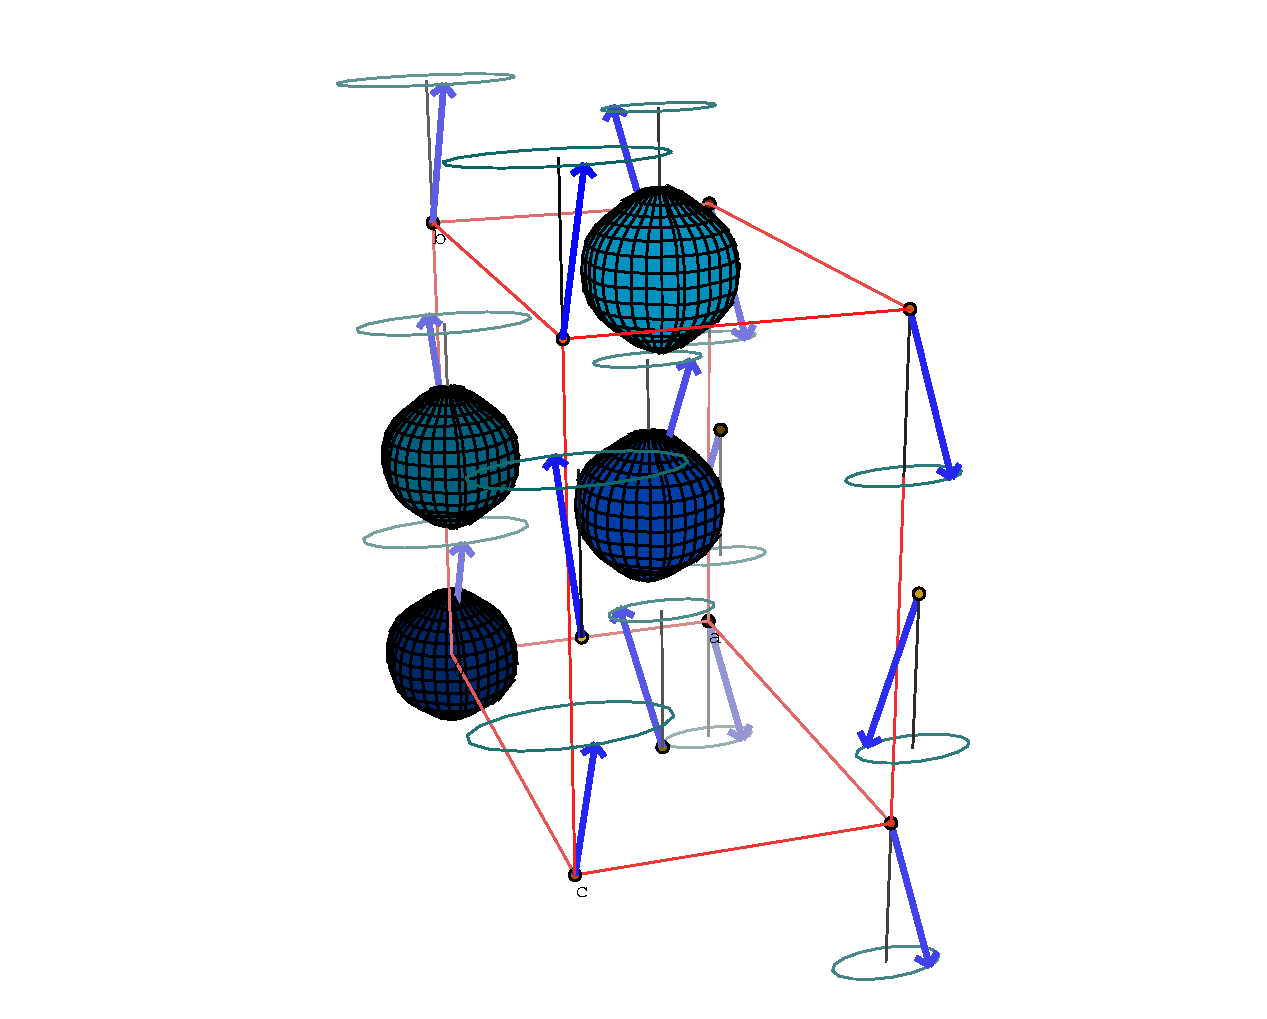
\includegraphics[angle=-0, width=0.6\textwidth]{figsrc/animationAF1.eps}
\end{center}
\caption{NdCu$_2$ - snapshot of animation of the mode 
at Q=(0.67 1 0) at energy 0.7~meV in phase AF1 at 
H=0 and T=1.5~K [plot created by program 
{\prg display\_chargedensities}\index{display\_chargedensities}]
}\label{animationAF1}
\end{figure}

\subsubsection{Graphical Visualization of Spin and Charge Oscillations of a Magnetic Excitation}

In addition to the calculation of the neutron scattering cross section, the dynamical susceptibility may be used to %%@
visualize the change of spin or chargedensity associated with such a magnetic excitation. By virtue of its definition %%@
this susceptibility describes the response (change $\Delta \langle J_{\alpha} \rangle$ of expectation values $\langle %%@
J_{\alpha}\rangle$) of the system to a spatial and time dependent magnetic field $H_{\beta}(\mbf R=\mbf R_{ijk}+\mbf %%@
r_{s'})=H^{s'}_{\beta}
\exp(i\mbf Q \mbf R-i\omega t)$ of frequency $\omega$ and wavevector $\mbf Q$:

\begin{equation}
\Delta \langle J^s_{\alpha}\rangle(\mbf Q,\omega)=\sum_{s'\beta}\chi^{ss'}_{\alpha\beta}(\mbf Q,\omega) H^{s'}_{\beta}
\end{equation} 

The corresponding oscillation of the moments in real space and time is given by 

\begin{equation}
\Delta \langle J^s_{\alpha}\rangle(\mbf R=\mbf R_{ijk}+\mbf r_s)=
\Delta \langle J^s_{\alpha}\rangle(\mbf Q,\omega)\exp(i\mbf Q \mbf R-i\omega t)=
\exp(i\mbf Q \mbf R-i\omega t) \sum_{s'\beta}\chi^{ss'}_{\alpha\beta}(\mbf Q,\omega) H^{s'}_{\beta}
\end{equation} 

We eliminate the sum in this equation by choosing the components of the applied field $H^{s'}_{\beta}=\epsilon %%@
\delta_{1s'}\delta{1\beta}$.
\begin{equation}\label{osc}
\Delta \langle J^s_{\alpha}\rangle(\mbf R=\mbf R_{ijk}+\mbf r_s)=
\exp(i\mbf Q \mbf R-i\omega t) \chi^{s1}_{\alpha1}(\mbf Q,\omega_r) \epsilon 
\end{equation} 

Due to the divergence of the susceptibility at the excitation  a small
applied field $\epsilon$ will induce a large oscillation amplitude of the moments, the amplitude
of the oscillation will depend on the relation of magnitude of the applied field $\epsilon$ and
the rate of damping of the magnetic excitation. Therefore we set the amplitude $a_0$ of the 
oscillation equal to $a_0=\epsilon / (\omega-\omega_r)$. Substituting this into (\ref{osc}) and
considering the susceptibility obtained from equation (\ref{psiresult}) etc. we obtain

\begin{equation}\label{oscill}
\Delta \langle J^s_{\alpha}\rangle(\mbf R=\mbf R_{ijk}+\mbf r_s)=
a_0 \exp(i\mbf Q \mbf R-i\omega_r t) 
\sqrt{\gamma^s}^\star \mathcal U^s_{\alpha1} \mathcal T_{sr}(\mbf Q) \omega_r \mathcal T^{\dag}_{r1}(\mbf Q) \mathcal %%@
U^{1\dag}_{11}\sqrt{\gamma^{1}}
\end{equation} 

This procedure is fine unless $\mathcal T^{\dag}_{r1}(\mbf Q)$ or $U^{1\dag}_{11}$ is zero. Therefore
it is convenient to redefine the amplitude $a=a_0 \mathcal T^{\dag}_{r1}(\mbf Q) \mathcal %%@
U^{1\dag}_{11}\sqrt{\omega_r\gamma^{1}}$.
We get

\begin{equation}\label{oscillation}
\Delta \langle J^s_{\alpha}\rangle(\mbf R=\mbf R_{ijk}+\mbf r_s)=
a \exp(i\mbf Q \mbf R-i\omega_r t) 
\sqrt{\omega_r\gamma^s}^\star \mathcal U^s_{\alpha1} \mathcal T_{sr}(\mbf Q)=
a \exp(i\mbf Q \mbf R-i\omega_r t) e^s_{r\alpha} 
\end{equation} 

The eigenvector components $e^s_{r\alpha}$ 
 of this oscillation are stored 
 in {\prg mcdisp.qev} and can be used bye program {\prg spins} to create
 a visualisation of the spin-oscillation (commands {\prg spins T Ha Hb Hc h k l E} and {\prg java javaview %%@
model=results/spins.*.jvx Animation.LastKey=16}). Note the in {\prg mcdisp.qev} the eigenvector components
for different $t$ in $s=(ijklt)$ (refering to different single ion transitions at the same ion $ijkl$) are summed up and 
therefore the format to store this information is the same as for a magnetic structure in {\prg mcphas.sps}.

I order to visualize a charge density the eigenvector $e^s_{r\alpha}$
 may be simply extended to $\alpha= 1,...,n,n+1,...N$ utilizing equation (\ref{ufirstrow})
  The index $\alpha' > 3$ refers
 to operators, which usually are not coupled by an interaction (however, they can be coupled
 by multipolar interactions, see section~\ref{qint}). The corresponding 
 oscillations of Stevens operator expectation values $\Delta \langle J_{\alpha = (nm)}\rangle(\mbf R=\mbf R_{ijk}+\mbf %%@
r_l) =\Delta \langle O_n^m(\mbf J_{ijkl})\rangle$ can be directly inserted into
(\ref{chargedensity_operator}) in order to evaluate the charge density oscillations. This is done by program
{\prg charges}, the commands are {\prg charges threshold T Ha Hb Hc h k l E} and {\prg java javaview %%@
model=results/charges.*.jvx Animation.LastKey=16}. Fig.~\ref{animationAF1} shows a snapshot of the result of such an %%@
animation (on screen both chargedensities and spins will move).





\begin{figure}[t]%h=here, t=top, b=bottom, p=separate figure page
\begin{center}\leavevmode
\includegraphics[angle=-0, width=0.6\textwidth]{figsrc/diffuse_ndcu2_10K.eps}
\end{center}
\caption{\label{diffus}
NdCu$_2$ - calculated diffuse magnetic scattering intensity in the (hk0) plane.
[plot created by program {\prg displaycontour\index{displaycontour}}]
}
\end{figure}

\subsection{Diffuse Scattering}

The program {\prg McDisp} may be used straightforward to calculate quasi elastic intensity
 by

\begin{itemize}
\item
 specification of an energy
range [emin,emax] in file {\prg mcdisp.par\index{mcdisp.par}} which corresponds to the interval of energies (around zero
energy transfer) sensed by the detector of the diffuse scattering experiment. 
\item
 using the option {\prg -r} forcing the program {\prg mcdisp\index{mcdisp}} to calculate the cross section
 using the full MF-RPA algorithm.
\item
 quasi elastic intensity is expected only in the paramagnetic state - thus in {\prg mcdisp.mf\index{mcdisp.mf}} a
 a temperature above the magnetic ordering temperature should be selected.
\end{itemize} 
 
The file {\prg mcdisp.dsigma.tot} produced by the calculation contains the calculated diffuse scattering cross section.
Figure~\ref{diffus} shows an output of such a calculation for the diffuse scattering
on NdCu$_2$.

\subsection{Going beyond the dipolar approximation in {\prg Mcdisp}}

In order to go beyond the dipolar approximation for inelastic scattering the formalism outlined in %%@
section~\ref{formalism}
has to be extended. The more general expression (\ref{dsdode}) for the inelastic neutron scattering cross section has to %%@
be used:

\begin{eqnarray}\label{dsdoderepeated}
\frac{d^2\sigma}{d\Omega dE'}&=&N\frac{k'}{k}\left( \frac{\hbar \gamma e^2}{m_e c^2}  \right)^2
%\sum_{\mbf Q} \delta_{\vec\kappa,\mbf Q}
\sum_{\alpha\beta}(\delta_{\alpha\beta}-\hat \mbf Q_{\alpha} \hat \mbf Q_{\beta}) 
S^{\alpha \beta}_{\rm mag}(\mbf Q,\omega)+
N\frac{k'}{k}S_{\rm nuc}(\mbf Q,\omega) \nonumber \\
S_{\rm mag}&=&S_{\rm mag}^{\rm el}+S_{\rm mag}^{\rm inel} \label{smag} 
\end{eqnarray}

The scattering function is given by

\begin{equation}
S_{\rm mag}^{\rm inel,\alpha\beta}(\mbf Q,\omega)=\frac{1}{2\pi\hbar}\int_{-\infty}^{+\infty}dt e^{i\omega t}
\frac{1}{N}\sum_{jj'} 
\times e^{-W_j(Q)- W_{j'}(Q)} e^{-i\mbf Q(\mbf R_j-\mbf R_{j'})}
(\langle \hat \mathcal Q^{j \dag}_{\alpha}(t) \hat \mathcal Q^{j'}_{\beta}(0) \rangle_{T,H}
- \langle \hat \mathcal Q^{j \dag}_{\alpha}\rangle_{T,H} \langle \hat \mathcal Q^{j'}_{\beta} \rangle_{T,H})
\end{equation}

In dipole approximation the scattering operator is written as a product of formfactor and inverse angular momentum %%@
operator~\footnote{
Note in case of intermediate coupling (''gJ=0'') the three components of the 
inverse total angular momentum operator are
substituted by the 6 components of inverse spin and orbital momentum
$\langle \hat \mathcal Q^{j}_{\alpha'}\rangle \sim 
\{\frac{1}{2} g_S F_S(Q)\}_j \langle J_{\alpha'}^j \rangle_{T,H} $ 
($\alpha' =a',c',e'$) and
$\langle \hat \mathcal Q^{j}_{\alpha'}\rangle \sim 
\{\frac{1}{2} g_L F_L(Q)\}_j \langle J_{\alpha'}^j \rangle_{T,H} $ 
($\alpha =b',d',f'$), $g_S=2,g_L=1$, $Ja'=S_a,Jb'=L_a$,
$Jc'=S_b,Jd'=L_b$,$Je'=S_c,Jf'=L_c$.
}  
$\langle \hat \mathcal Q^{j}_{\alpha}\rangle \sim \{\frac{1}{2} g_J F(Q)\}_j \langle J_{\alpha}^j \rangle_{T,H} $ and %%@
the
cross section may be rewritten using the scattering function $S_{ss'}^{\alpha\beta}({\mbf Q},\omega)$ as done
in equation~(\ref{int}), note the sum over positions $j$ is split into a sum over lattice vectors ($\mbf G_l$)
and the basis of the magnetic unit cell ($\mbf B_s$) 

\begin{equation}
S_{ss'}^{\alpha\beta}({\mbf Q},\omega)=\int_{-\infty}^{+\infty}dt e^{i\omega t}e^{-i\mbf Q(\mbf B_s-\mbf B_{s'})}
\frac{1}{N_g}\sum_{ll'}e^{-i\mbf Q(\mbf G_l-\mbf G_{l'})}
(\langle  J^{sl \dag}_{\alpha}(t)  J^{s'l'}_{\beta}(0) \rangle_{T,H}
- \langle  J^{sl \dag}_{\alpha}\rangle_{T,H} \langle J^{s'l'}_{\beta} \rangle_{T,H})
\end{equation}

Going beyond the dipole approximation, another scattering function $\Sigma_{ss'}^{\alpha\beta}({\mbf Q},\omega)$
is introduced, which is obtained from $S_{ss'}^{\alpha\beta}({\mbf Q},\omega)$ by substituting
the angular momentum operators $\mbf J$ with the scattering operators $\mathcal Q$.

\begin{equation}
\Sigma_{ss'}^{\alpha\beta}({\mbf Q},\omega)=\int_{-\infty}^{+\infty}dt e^{i\omega t}e^{-i\mbf Q(\mbf B_s-\mbf B_{s'})}
\frac{1}{N_g}\sum_{ll'}e^{-i\mbf Q(\mbf G_l-\mbf G_{l'})}
(\langle \hat \mathcal Q^{sl \dag}_{\alpha}(t) \hat \mathcal Q^{s'l'}_{\beta}(0) \rangle_{T,H}
- \langle \hat \mathcal Q^{sl \dag}_{\alpha}\rangle_{T,H} \langle \hat \mathcal Q^{s'l'}_{\beta} \rangle_{T,H})
\end{equation}

Using this function the inelastic magnetic neutron scattering cross section can be rewritten as

\begin{eqnarray}\label{intbeyond}
\frac{d \sigma_{\rm mag}^{\rm inel}}{d\Omega dE'}&=&N \frac{k'}{k} \left(\frac{\hbar \gamma e^2}{m_e c^2}\right)^2
%\sum_{\mbf Q} \delta_{\vec\kappa,\mbf Q}
\sum_{\begin{array}{c} \alpha \beta \\ s s' \\ \end{array}}
(\delta_{\alpha\beta}-\hat Q_{\alpha} \hat Q_{\beta})
e^{-W_s(Q)- W_{s'}(Q)} 
\frac{\Sigma_{ss'}^{\alpha\beta}({\mbf Q},\omega)}{2\pi \hbar N_b}  
\end{eqnarray}

Note that also to this scattering function the fluction dissipation theorem can be applied relating
$\Sigma$ to a dynamical susceptibility $X$: 

\begin{eqnarray}\label{fluctdissbeyond}
\Sigma_{ss'}^{\alpha\beta}({\mbf Q},\omega) &=&
\frac{2 \hbar}{1-e^{-\hbar\omega/kT}} X_{\alpha\beta}^{,,ss'}({\mbf Q},\omega) \\ \nonumber
X_{\alpha\beta}^{,,ss'}({\mbf Q},\omega)&=&
\frac{1}{2i}\left[
X_{\alpha\beta}^{ss'}({\mbf Q},\omega)-
X_{\beta\alpha}^{*s's}({\mbf Q},\omega)
\right]
\end{eqnarray}

However, in contrast to the conventional dynamical susceptibility 
$\chi_{\alpha\beta}^{ss'}({\mbf Q},\omega)$
 this new susceptibility
cannot be obtained from solving the MF-RPA equation (\ref{mfrpa}), because the derivation of (\ref{mfrpa})
makes use of the dynamical evolution of the angular momentum and not of the scattering operator. 

However, general properties of dynamical susceptibilities may be used 
to get a relation between
$X_{\alpha\beta}^{ss'}({\mbf Q},\omega)$ and 
$\chi_{\alpha\beta}^{ss'}({\mbf Q},\omega)$, which may be used.  In general a dynamical susceptibility %%@
$\chi_{BA}(\omega)$ describes the response of
 a physical observable $\langle \hat B(t)\rangle$ to a perturbation of the system described by 
an operator $\hat A$.
In the case of $\chi_{\alpha\beta}^{ss'}({\mbf Q},\omega)$ we have 
$\hat A=\frac{1}{\sqrt{N_g}}e^{i\mbf B_{s'}}\sum_{l'}e^{i\mbf Q\mbf G_{l'}}J^{s'l'}_{\beta}$,
$\hat B=\frac{1}{\sqrt{N_g}}e^{i\mbf B_{s}}\sum_{l}e^{i\mbf Q\mbf G_{l}}J^{sl}_{\alpha}$.
In the case of $X_{\alpha\beta}^{ss'}({\mbf Q},\omega)$ we have 
$\hat A=\frac{1}{\sqrt{N_g}}e^{i\mbf B_{s'}}\sum_{l'}e^{i\mbf Q\mbf G_{l'}}\hat \mathcal Q^{s'l'}_{\beta}$,
$\hat B=\frac{1}{\sqrt{N_g}}e^{i\mbf B_{s}}\sum_{l}e^{i\mbf Q\mbf G_{l}}\hat \mathcal Q^{sl}_{\alpha}$.

From linear response theory it can be shown~\cite[page 143]{jensen91-1}, that the dynamical susceptibilities have poles %%@
at the excitation energies of the system:

\begin{equation}\label{gensus}
\chi_{BA}= \lim_{\epsilon \rightarrow 0^+}\sum_{\alpha\alpha'}\frac{\langle \alpha |\hat B|\alpha' \rangle 
\langle \alpha' |\hat A|\alpha \rangle }{E_{\alpha'}-E_{\alpha}-\hbar \omega - i \hbar \epsilon}(p_{\alpha}-p_{\alpha'})
\end{equation}
 
The denominator, the eigenstates and the difference in thermal population are the same for any susceptibility.
The energy eigenstates $|\alpha \rangle$ of the system will be a linear combination of products of 
single ion states. 
Therefore, the numerator in equation (\ref{gensus}) will 
be a (usually not known) linear combination of products of the form 
$\langle -|J_{\alpha}^s|+\rangle \langle +'|J_{\beta}^{s'}|-'\rangle$ 
and 
$\langle -|\hat \mathcal Q_{\alpha}^s|+\rangle \langle +'|\hat \mathcal Q_{\beta}^{s'}|-'\rangle$ for
 $\chi_{\alpha\beta}^{ss'}({\mbf Q},\omega)$ and 
   $X_{\alpha\beta}^{ss'}({\mbf Q},\omega)$, respectively.

These terms can be related by a similar procedure as 
outlined in equations (\ref{mmatrix}) ff:

\begin{eqnarray}\label{mumatrix}
\mu^s_{\alpha\beta}=\langle -|J^{s}_{\alpha}|+\rangle\langle +|J^s_{\beta}|-\rangle \\
\nu^s_{\alpha\beta}=\langle -|\mathcal Q^{s \dag}_{\alpha}|+\rangle\langle +|\mathcal Q^s_{\beta}|-\rangle
\end{eqnarray}

similar to $M_{\alpha\beta}^s$ the matrices  $\mu_{\alpha\beta}^s$ and $\nu_{\alpha\beta}^s$ 
can be diagonalised using the
unitary transformations $\overline \mathcal  U_{\alpha\beta}^s$ (${\overline \mathcal U^{s\dag}\overline \mathcal U^s}=1$) and
$\overline \mathcal V_{\alpha\beta}^s$ (${\overline \mathcal V^{s\dag}\overline \mathcal V^s}=1$), respectively. Note that in the case $\langle +| \neq \langle -|$
the unitary transformations $\overline \mathcal U =\mathcal U$ and $\overline \gamma = \gamma$.

\begin{equation}
\overline \gamma^s=(p_--p_+)\sum_{\alpha}\langle -|J^s_{\alpha}|+\rangle\langle +|J^s_{\alpha}|-\rangle
\end{equation}


Thus we have for orthogonal states 

\begin{eqnarray}
\langle -|         J^{s     }_{\alpha}|+\rangle\langle +|         J^s_{\beta}|-\rangle&=&\overline \mathcal U_{\alpha 1}^s\phi^s\overline \mathcal U_{1\beta}^{s\dag} \dots %%@
{\rm with }\, \phi^s=\overline \gamma^s/(p_--p_+)\\
\langle -|\mathcal Q^{s \dag}_{\alpha}|+\rangle\langle +|\mathcal Q^s_{\beta}|-\rangle&=&\overline \mathcal V_{\alpha 1}^s\xi^s\overline \mathcal V_{1\beta}^{s\dag}  
\end{eqnarray}

Multiplying this from the right(left) side with 
$\overline \mathcal U_{\beta\beta'}^{s}/\sqrt(\phi^s)$
($\overline \mathcal U_{\alpha'\alpha}^{s\dag}/\sqrt(\phi^s)^{\star}$)
and summing over $\beta$ ($\alpha$) we get

\begin{equation}
\frac{1}{\phi^s}\left ( \sum_{\alpha}\overline \mathcal U_{\alpha'\alpha}^{s\dag} \langle -|         J^{s     }_{\alpha}|+\rangle \right )
\left ( \sum_{\beta} \langle +|         J^s_{\beta}|-\rangle\overline \mathcal U_{\beta\beta'}^{s} \right )
= \delta_{1\alpha'} \delta_{1\beta'}
\end{equation}

It follows

\begin{equation}
\frac{1}{\sqrt{\phi^s}}
\left ( \sum_{\alpha}\overline \mathcal U_{\alpha'\alpha}^{s\dag} \langle -|         J^{s     }_{\alpha}|+\rangle \right )
= \delta_{1\alpha'}
\end{equation}

Using these properties of the unitary transformation we can transform any product
$\langle -|J_{\alpha}^s|+\rangle \langle +'|J_{\beta}^{s'}|-'\rangle$ 
in the numerator of (\ref{gensus}) to $\delta_{1\alpha'} \delta_{1\beta'}$:

\begin{equation}\label{trafo1}
\left ( \sum_{\alpha}\frac{1}{\sqrt{\phi^s}^{\star}}\overline \mathcal U_{\alpha'\alpha}^{s\dag} \langle -|J^{s}_{\alpha}|+\rangle \right )
\left ( \sum_{\beta} \langle +'|J^{s'}_{\beta}|-'\rangle \frac{1}{\sqrt{\phi^{s'}}}\overline \mathcal U_{\beta\beta'}^{s'} \right )
= \delta_{1\alpha'} \delta_{1\beta'}
\end{equation}

Further transformation with 
$\sum_{\alpha'}\overline \mathcal V_{\alpha''\alpha'}^{s} \sqrt{\xi^s}^{\star}$ and
$\sum_{\beta'} \sqrt{\xi^{s'}}\overline \mathcal V_{\beta'\beta''}^{s' \dag} $ transforms the term to
$\langle -|\hat \mathcal Q_{\alpha''}^s|+\rangle \langle +'|\hat \mathcal Q_{\beta''}^{s'}|-'\rangle$,
i.e.

\begin{equation}\label{trafo2}
\sum_{\alpha'\beta'}\overline \mathcal V_{\alpha''\alpha'}^{s} \sqrt{\xi^s}^{\star}\delta_{1\alpha'} \delta_{1\beta'}
 \sqrt{\xi^{s'}}\overline \mathcal V_{\beta'\beta''}^{s' \dag}=
\langle -|\hat \mathcal Q_{\alpha''}^s|+\rangle \langle +'|\hat \mathcal Q_{\beta''}^{s'}|-'\rangle
\end{equation}

Applying the two set of transformations (\ref{trafo1}) and (\ref{trafo2}) to
the dynamical susceptibility $\chi_{\alpha\beta}^{ss'}({\mbf Q},\omega)$ we
obtain $X_{\alpha''\beta''}^{ss'}({\mbf Q},\omega)$: 

\begin{equation}\label{finalslow}
X_{\alpha''\beta''}^{,,ss'}({\mbf Q},\omega)=\sum_{\alpha\alpha'\beta\beta'}
\sqrt{\frac{\Gamma^s}{\overline \gamma^s}}^{\star}
\overline \mathcal V_{\alpha''\alpha'}^{s}
 \overline  \mathcal U_{\alpha'\alpha}^{s\dag} 
    \chi_{\alpha\beta}^{,,ss'}({\mbf Q},\omega)
 \overline  \mathcal U_{\beta\beta'}^{s'} 
 \overline \mathcal V_{\beta'\beta''}^{s' \dag}
\sqrt{\frac{\Gamma^{s'}}{\overline \gamma^{s'}}}
\end{equation}

(Note here we have defined $\Gamma^s \equiv \xi^s(p_--n+)$).
Having obtained the dynamical susceptibility $    \chi_{\alpha\beta}^{,,ss'}({\mbf Q},\omega)$
by the method outlined in section \ref{formalism}, 
the expression (\ref{finalslow})
 can be inserted in (\ref{intbeyond}) and (\ref{fluctdissbeyond})  to evaluate 
the neutron scattering cross section numerically.
{\small Technically, the single ion module has to provide in addition to the
matrices $M^s_{\alpha\beta}$ (equation (\ref{mmatrix})) for every $\mbf Q$-vector
the vector 
$\sqrt{\Gamma^s}^\star \overline \mathcal V^s_{\alpha1}\equiv
 {\mbf v^s_{\alpha1}}(\mbf Q)=\sqrt{(p_--p_+)}\langle -|\mathcal Q^{\dag}_{\alpha}|+\rangle$, which will depend on the 
scattering vector $\mbf Q$.}

For the DMD algorithm we insert  (\ref{dmdfinal}) into (\ref{finalslow}) and obtain


\begin{equation}\label{Xcalc}
X^{,,ss'}_{\alpha\beta}(\mbf Q,\omega)=\sqrt{\Gamma^s}^\star\sqrt{\Gamma^{s'}} 
\pi \sum_r 
 \mathcal V^s_{\alpha1} \mathcal T_{sr}(\mbf Q)\omega_r(\mbf Q) \delta(\hbar \omega_r(\mbf Q) %%@
- \hbar \omega) \mathcal T^{\dag}_{rs'}(\mbf Q)  \mathcal V^{s'\dag}_{1\beta}
\end{equation}

with 

\begin{equation}
 \mathcal V^s_{\alpha1} =\sqrt{\frac{\gamma^s}{\overline \gamma^s}}^{\star}\sum_{\alpha'\alpha''} \overline \mathcal V_{\alpha\alpha'}^s \overline \mathcal U^{s\dag}_{\alpha'\alpha''}
\mathcal U^s_{\alpha''1}
\end{equation}

If $\langle +|\neq\langle -|$ then $\overline \mathcal V=\mathcal V$.

{\prg mcdisp\index{mcdisp}} automatically calculates the intensity in
dipole approximation and also going beyond, if possible, the result
is stored in file {\prg mcdisp.qei}.

\subsection{Powder Neutron Cross Section}


\begin{figure}[tb]%h=here, t=top, b=bottom, p=separate figure page
\begin{center}\leavevmode
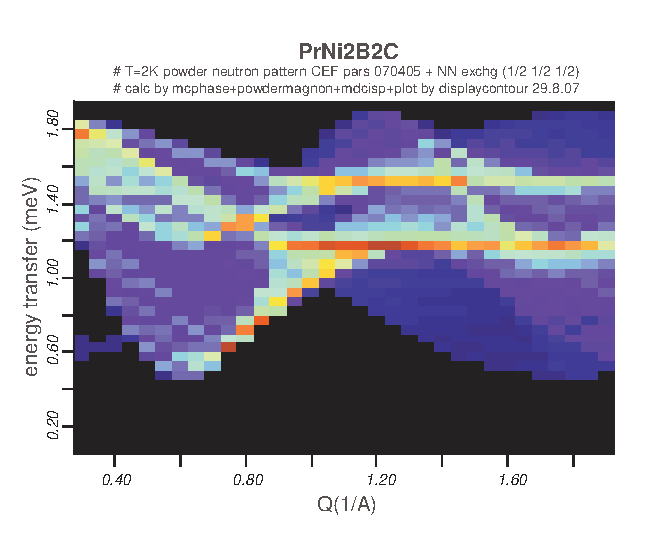
\includegraphics[angle=0, width=0.5\textwidth]{figsrc/contour2K_070504.eps}
\end{center}
\caption{Magnetic Neutron powder spectrum of PrNi$_2$B$_2$C for $T=2$~K as calculated using module {\prg powdermagnons} %%@
in combination with {\prg 
mcdisp}.}\label{prni2b2c_2K}
\end{figure}

\begin{figure}[tb]%h=here, t=top, b=bottom, p=separate figure page
\begin{center}\leavevmode
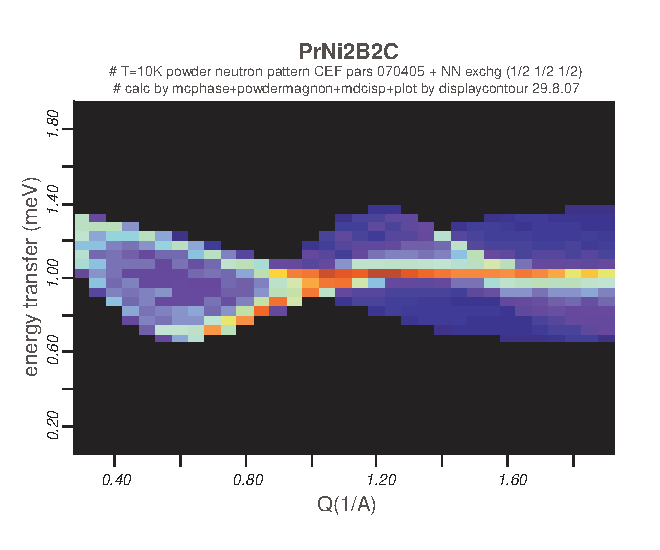
\includegraphics[angle=0, width=0.5\textwidth]{figsrc/contour10K_070504.eps}
\end{center}
\caption{Magnetic Neutron powder spectrum of PrNi$_2$B$_2$C for $T=10$~K  as calculated using module {\prg %%@
powdermagnons} in combination with {\prg 
mcdisp}.}\label{prni2b2c_10K}
\end{figure}

{\prg Mcdisp} in combination with module {\prg powdermagnon} can be used to calculate
powder neutron pattern. In order to do this, a 3-step procedure is required:

\subsubsection{Creation of the q-vector list}
The first step is to create a list of reflections to be used for 
the averaging of the powder neutron cross section. 

just type: powdermagnon 0.3 2 0.1 80

meaning take file {\prg mcphas.j\index{mcphas.j}}, generate a reflection list and put it to 
file {\prg mcdisp.par\index{mcdisp.par}}. Parameters are 
\begin{itemize}
\item
 0.3 ....qmin   [1/A] minimal q vector
\item
 2   ....qmax   [1/A] maximal q vector
\item
 0.1 ....deltaq [1/A] step width in q
\item
 80  ....number of steps in polar coordinate $\Theta$
        (steps in polar angle $\phi$ are  then calculated in module
        {\prg powdermagnon} by $\delta \phi= \delta \Theta*\pi/(4*sin(\Theta))$
\end{itemize}

\subsubsection{Calculation of the Dispersion using {\prg mcdisp\index{mcdisp}}}

In order to set the correct temperature and $k_f$ (or $k_i$) etc. edit
the input files for module {\prg mcdisp\index{mcdisp}} and start {\prg mcdisp\index{mcdisp}}. Mind 
to select the fast algorithm so that a file {\prg mcdisp.qei} is created.

\subsubsection{Powder-averaging the spectra}
The third and last step in the calculation of the powder pattern is the averaging
of the spectra with the same value of $Q$. This is done by restarting module
{\prg powdermagnon} by: 

powdermagnon -r results\\mcdisp.qei 0.5 30 0.2 

meaning take  results from file {\prg results\\mcdisp.qei} and average the
spectra. Output is printed to the console (STDOUT) and can be piped to a file in
order to print it with {\prg displaycontour\index{displaycontour}}. An example is given in fig.~
\ref{prni2b2c_2K} and \ref{prni2b2c_10K}.
Parameters in the command line are:
\begin{itemize}
\item 0.5 ....Emin   [meV] minimal energy
\item 0.5 ....Emax   [meV] maximal energy
\item 0.5 ....deltaE [meV] energy step width
\end{itemize}
